\subsection{Principle Component Analysis}
The Principle Components Analysis (PCA) is an tool that can be used to describe the variance in a data set.

PCA aims to reduce the number of dimension used to represent the features of the data.
This is done by finding the eigenvectors and eigenvalues to the training set.
These represent a new rotated and translated coordinate axis, sorted from the one with the highest variance to the lowest.
The least significant components can then be removed.
Thus efficiently reducing the dimensions, but still keeping the most significant features in the data.

In figure \ref{fig:variance} is the variance and accumulated variance shown for the first 20 principle components (PC). 
It is seen that the first PC is the most significant and the variance converges towards zero with more PC.

\begin{figure}[H]
\centering
\begin{subfigure}{0.70\textwidth}
\centering
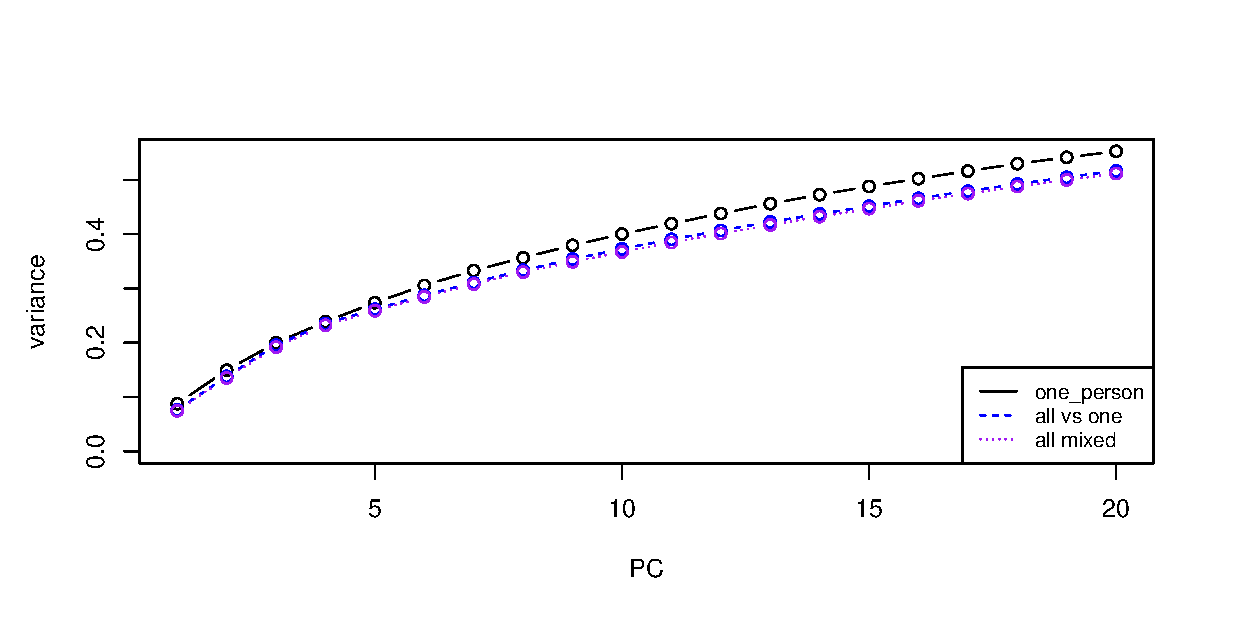
\includegraphics[width=\textwidth]{graphics/pca_acc_variance}
\caption{Accumulated variance.}
\label{fig:pca_accumulated_var}
\end{subfigure}\\[-1cm]
\end{figure}
\begin{figure}[H]
\centering
\ContinuedFloat
\begin{subfigure}{0.70\textwidth}
\centering
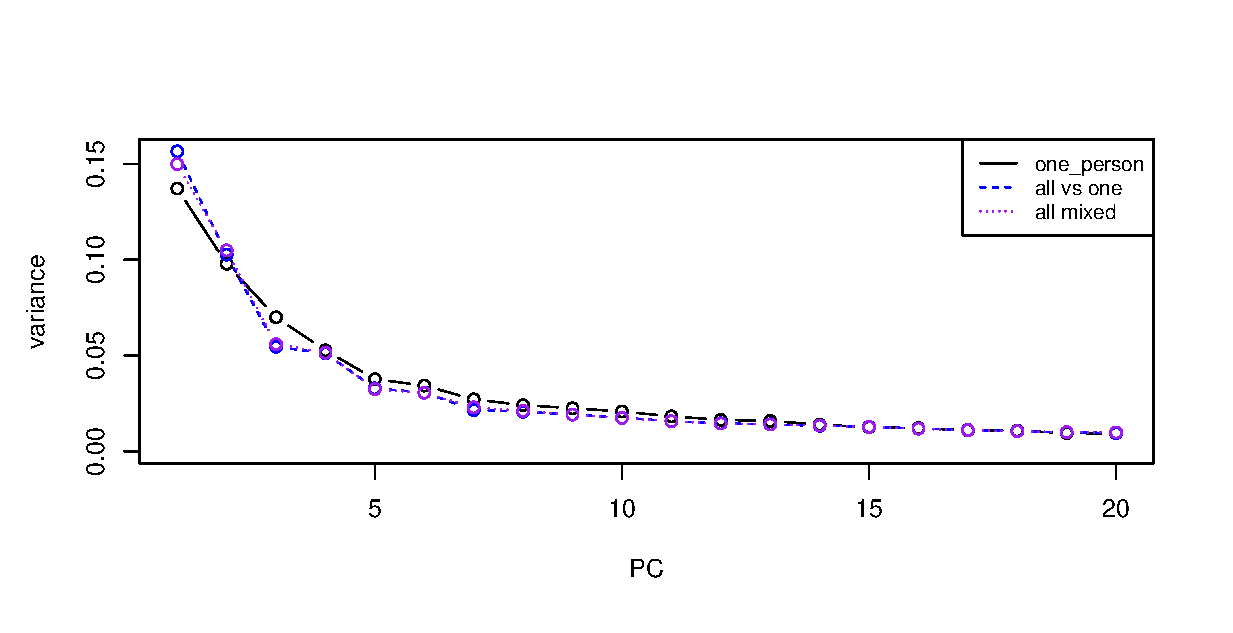
\includegraphics[width=\textwidth]{graphics/pca_variance}
\caption{Variance of a single component.}
\label{fig:pca_var}
\end{subfigure}
\caption[PCA variance.]{Variance for the first 20 principle components.
The data was run on Group 3 member 2's data on 100 DPI. }
\label{fig:variance}
\end{figure}
% Figure \ref{fig:contour_KvsPCA_G3M2vsRest} shows a contour plot of how well Group 3 Member 2's  handwriting was predicted successfully for $K$ and the total variance represented of the PC's varying between one and 20 and 0.5 and 1 respectively.


The variance can also be plotted using the same data, but normalized using z-score first.
This is illustrated on figure \ref{fig:variance_zscore}.




\begin{figure}[H]
\centering
\begin{subfigure}{0.70\textwidth}
\centering
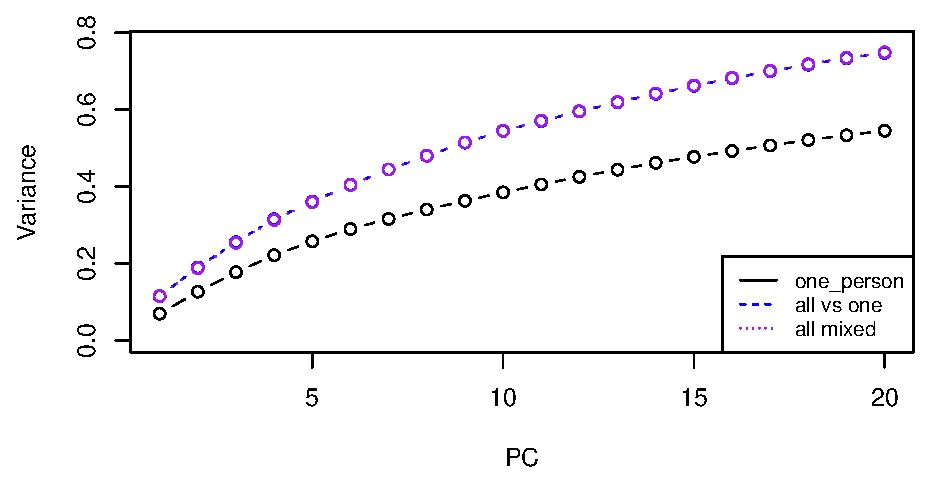
\includegraphics[width=\textwidth]{graphics/pca_acc_variance_zs}
\caption{Accumulated variance.}
\label{fig:pca_accumulated_var_zscore}
\end{subfigure}\\[-1cm]
\begin{subfigure}{0.70\textwidth}
\centering
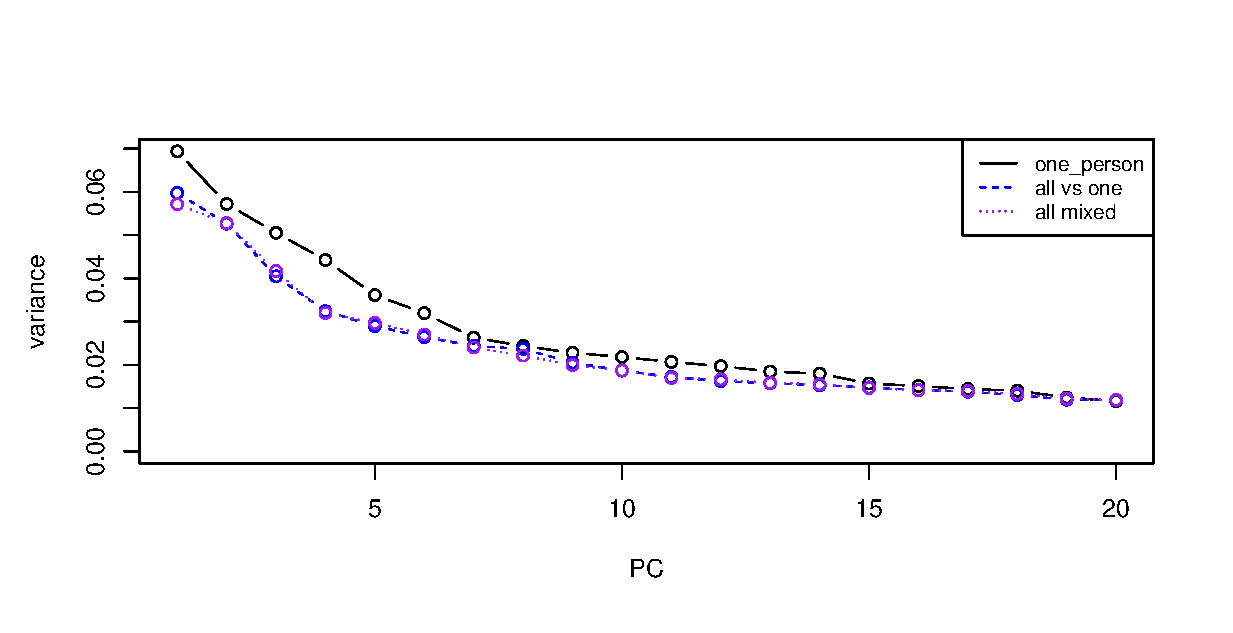
\includegraphics[width=\textwidth]{graphics/pca_variance_zs}
\caption{Variance of a single component.}
\label{fig:pca_var_zscore}
\end{subfigure}
\caption[PCA variance when data is normalized using z-score.]{Variance for the first 20 principle components on a z-score normalized dataset.
The data was run on Group 3 member 2's data on 100 DPI. }
\label{fig:variance_zscore}
\end{figure}

\todo[inline]{Remove padding in these files. It looks like caption a is the title of figure b.}


The effect of using z-score can be seen in figure \ref{fig:variance_zscore}.
It is clear that the variance of the first PC in figure \ref{fig:pca_var} is considerably higher than that of figure \ref{fig:pca_var_zscore} for all three tests.
As the number of components increases, the two curves for the one-person test catches up to the higher in figure \ref{fig:pca_accumulated_var_zscore} which was not normalized.
However, the results for the two other test sets show that the accumulative variance in the case of using z-score averages the variance amongst the components more.
This results in the first few components being less significant than when not using z-score, but the lower PC have a higher level of significance.
Furthermore a larger set of PC are necessary to represent the same variance when using PCA with z-score applied beforehand than when not using it.



